\documentclass[UTF8, 12pt]{ctexart}
% UTF8编码,ctexart现实中文
\usepackage{color}
% 使用颜色
\definecolor{orange}{RGB}{255,127,0} 
\definecolor{violet}{RGB}{192,0,255} 
\definecolor{aqua}{RGB}{0,255,255} 
\usepackage{geometry}
\setcounter{tocdepth}{5}
\setcounter{secnumdepth}{5}
% 设置五级目录与标题
\geometry{papersize={21cm,29.7cm}}
% 默认大小为A4
\geometry{left=3.18cm,right=3.18cm,top=2.54cm,bottom=2.54cm}
% 默认页边距为1英尺与1.25英尺
\usepackage{indentfirst}
\setlength{\parindent}{2.45em}
% 首行缩进2个中文字符
\usepackage{setspace}
\renewcommand{\baselinestretch}{1.5}
% 1.5倍行距
\usepackage{amssymb}
% 因为所以
\usepackage{amsmath}
% 数学公式
\usepackage[colorlinks,linkcolor=black,urlcolor=blue]{hyperref}
% 超链接
\usepackage{tikz}
% 绘图
\usepackage{unicode-math}
% 二重闭合积分
\author{Didnelpsun}
\title{多元函数积分学}
\date{}
\begin{document}
\maketitle
\pagestyle{empty}
\thispagestyle{empty}
\tableofcontents
\thispagestyle{empty}
\newpage
\pagestyle{plain}
\setcounter{page}{1}
\section{二重积分}

\subsection{概念}

\subsubsection{几何背景}

二重积分的几何背景就是曲顶柱体的体积。定积分用极限的思想求出了二维平面的曲边梯形的面积,同样二重积分$\iint\limits_Df(x,y)\,\textrm{d}\sigma$。

被积函数$f(x,y)$作为曲顶柱体在点$(x,y)$处柱体微元的高,用底面积$\textrm{d}\sigma>0$乘上高$f(x,y)$就得到一个小柱体体积,再把所有$D$上的柱体相加起来就是整个曲顶柱体的体积。

\subsubsection{性质}

\begin{itemize}
    \item 求区域面积:$\iint\limits_D1\cdot\textrm{d}\sigma=\iint\limits_D\textrm{d}\sigma=A$,其中$A$为$D$的面积。
    \item 可积函数必有界:当$f(x,y)$在有界闭区间$D$上可积时,$f(x,y)$在$D$上必有界。
    \item 积分线性性质:$k_1,k_2$为常数,则$\iint\limits_D[k_1f(x,y)\pm k_2g(x,y)]\,\textrm{d}\sigma=\iint\limits_{D_1}f(x,y)\,\textrm{d}\sigma$\\$\pm k_2\iint\limits_{D_2}f(x,y)\,\textrm{d}\sigma$。
    \item 积分可加性:当$f(x,y)$在有界闭区间$D$上可积时,且$D_1\cup D_2=D$,$D_1\cap U_2=\varnothing$,则$\iint\limits_Df(x,y)\,\textrm{d}\sigma=\iint\limits_{D_1}f(x,y)\,\textrm{d}\sigma+\iint\limits_{D_2}f(x,y)\,\textrm{d}\sigma$。
    \item 积分保号性:当$f(x,y),g(x,y))$在有界闭区间$D$上可积时,若在$D$上有$f(x,y)\leqslant g(x,y)$,则$\iint\limits_Df(x,y)\,\textrm{d}\sigma\leqslant\iint\limits_Dg(x,y)\,\textrm{d}\sigma$,特别$\left\vert\iint\limits_Df(x,y)\,\textrm{d}\sigma\right\vert\leqslant\iint\limits_D\vert f(x,y)\vert\,\textrm{d}\sigma$。
    \item 二重积分估值定理:设$M,m$,分别为$f(x,y)$在有界闭区域$D$上的最大值和最小值,$A$为$D$的面积,则有$mA\leqslant\iint\limits_Df(x,y)\,\textrm{d}\sigma\leqslant MA$。
    \item 二重积分中值定理:设函数$f(x,y)$在有界闭区域$D$上连续,$A$为$D$的面积,则在$D$上至少存在一点$(\xi,\eta)$使得$\iint\limits_Df(x,y)\,\textrm{d}\sigma=f(\xi,\eta)A$。
\end{itemize}

\textbf{例题:}设$I_1=\iint\limits_D\cos\sqrt{x^2+y^2}\,\textrm{d}\sigma$,$I_2=\iint\limits_D\cos(x^2+y^2)\,\textrm{d}\sigma$,$I_3=\iint\limits_D\cos(x^2+y^2)^2\,\textrm{d}\sigma$,其中$D=\{(x,y)|x^2+y^2\leqslant1\}$,则()。

$A.I_3>I_2>I_1$\qquad$B.I_1>I_2>I_3$\qquad$C.I_2>I_1>I_3$\qquad$D.I_3>I_1>I_2$

解:令$x^2+y^2=t$,$\therefore0<t\leqslant1$。所以$1\geqslant\sqrt{t}\geqslant t\geqslant t^2\geqslant0$。

又$\cos x$单调减,所以$A$。

\subsubsection{对称性}

普通对称性\textcolor{violet}{\textbf{定义:}}设$D$关于$y$轴对称,$I=\iint\limits_Df(x,y)\,\textrm{d}\sigma$,将$D$分为对称的两部分$D_1D_2$,即$I=\left\{\begin{array}{ll}
    2\iint\limits_{D_1}f(x,y)\,\textrm{d}\sigma, & f(x,y)=f(-x,y) \\
    0, & f(x,y)=-f(-x,y)
\end{array}\right.$。关于$x$轴对称也同理。

轮换对称性\textcolor{violet}{\textbf{定义:}}$xy$对调后区域$D$不变或关于$y=x$对称,$\iint\limits_Df(x,y)\,\textrm{d}x\textrm{d}y$\\$=\iint\limits_Df(y,x)\,\textrm{d}y\textrm{d}x$。类似积分值与积分变量无关。同理对于一元函数积分的不变性:$\int_a^bf(x)\,\textrm{d}x=\int_a^bf(y)\,\textrm{d}y$。

\textbf{例题:}设区域$D=\{(x,y)|x^2+y^2\leqslant1,x\geqslant0,y\geqslant0\}$,$f(x)$在$D$上的正值连续函数,$a,b$为常数,求$I=\displaystyle{\iint\limits_D\dfrac{a\sqrt{f(x)}+b\sqrt{f(y)}}{\sqrt{f(x)}+\sqrt{f(y)}}\textrm{d}\sigma}$。

解:由于被积函数是抽象的,所以无法直接计算。但是由于$D$是圆,$xy$对调后$D$保持不败你,所以$D$关于$y=x$对称,根据轮换对称性:\medskip

$I=\displaystyle{\iint\limits_D\dfrac{a\sqrt{f(x)}+b\sqrt{f(y)}}{\sqrt{f(x)}+\sqrt{f(y)}}\textrm{d}\sigma=\iint\limits_D\dfrac{a\sqrt{f(y)}+b\sqrt{f(x)}}{\sqrt{f(y)}+\sqrt{f(x)}}\textrm{d}\sigma}$。

$\therefore2I=\displaystyle{\iint\limits_D\dfrac{a\sqrt{f(x)}+b\sqrt{f(y)}}{\sqrt{f(x)}+\sqrt{f(y)}}\textrm{d}\sigma+\iint\limits_D\dfrac{a\sqrt{f(y)}+b\sqrt{f(x)}}{\sqrt{f(y)}+\sqrt{f(x)}}\textrm{d}\sigma}=\iint\limits_D(a+b)\,\textrm{d}\sigma$\\$=(a+b)\dfrac{\pi}{4}$。

解得$I=\dfrac{a+b}{8}\pi$。

\subsection{计算}

\subsubsection{直角坐标系}

后积先定限,先内画条线,先交写下限,后交写上限。

\paragraph{\texorpdfstring{$X$}型区域} \leavevmode \medskip

\begin{minipage}{0.6\linewidth}
    也称为上下型区域。

    $\iint\limits_Df(x,y)\,\textrm{d}\sigma=\int_a^b\textrm{d}x\int_{\psi(x)}^{\phi(x)}f(x,y)\,\textrm{d}y$。
\end{minipage}
\hfill
\begin{minipage}{0.3\linewidth}
    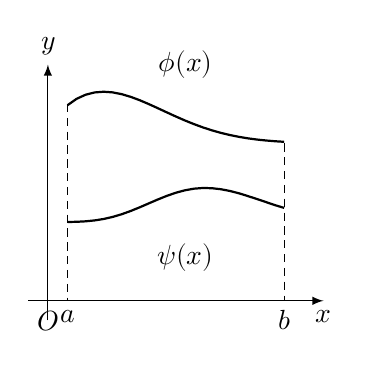
\begin{tikzpicture}[scale=1]
        \draw[-latex](-0.25,0) -- (3.5,0) node[below]{$x$};
        \draw[-latex](0,-0.25) -- (0,3) node[above]{$y$};
        \filldraw[black] (0,0) node[below]{$O$};
        \draw[black, thick, domain=0.25:3] plot (\x,{pow(\x,0.5)*pow(e,-\x*\x/2)+2});
        \filldraw[black] (1.75,3) node{$\phi(x)$};
        \draw[black, thick, domain=0.25:3] plot (\x,{pow(\x,4)*pow(e,-\x*\x/2)/5+1});
        \filldraw[black] (1.75,0.55) node{$\psi(x)$};
        \draw[black, densely dashed](0.25,2.5) -- (0.25,0) node[below]{$a$};
        \draw[black, densely dashed](3,2) -- (3,0) node[below]{$b$};
    \end{tikzpicture}
\end{minipage}

\paragraph{\texorpdfstring{$Y$}型区域} \leavevmode \medskip

\begin{minipage}{0.3\linewidth}
    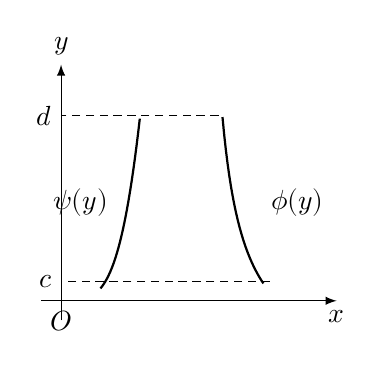
\begin{tikzpicture}[scale=1]
        \draw[-latex](-0.25,0) -- (3.5,0) node[below]{$x$};
        \draw[-latex](0,-0.25) -- (0,3) node[above]{$y$};
        \filldraw[black] (0,0) node[below]{$O$};
        \draw[black, thick, domain=2.05:2.57] plot (\x,{pow(\x-1.75,-1)-1});
        \filldraw[black] (3,1.25) node{$\phi(y)$};
        \draw[black, thick, domain=0.5:1] plot (\x,{pow(\x+0.25,6)*pow(e,-\x*\x/2)});
        \filldraw[black] (0.25,1.25) node{$\psi(y)$};
        \draw[black, densely dashed](2.65,0.25) -- (0,0.25) node[left]{$c$};
        \draw[black, densely dashed](2,2.35) -- (0,2.35) node[left]{$d$};
    \end{tikzpicture}
\end{minipage}
\hfill
\begin{minipage}{0.5\linewidth}
    也称为左右型区域。

    $\iint\limits_Df(x,y)\,\textrm{d}\sigma=\int_c^d\textrm{d}y\int_{\psi(y)}^{\phi(y)}f(x,y)\,\textrm{d}x$。
\end{minipage}

\paragraph{区域类型选择} \leavevmode \medskip

若上下是两条曲线,那么就是$X$型,若左右是两条曲线,那么就是$Y$型。

若同一个方向的函数有两种不同的表达式,则从另一个方向将$D$按照函数分段割开求积分。

\subsubsection{极坐标系}

按积分区域与极点位置关系的不同,将二重积分计算分为三种情况:

根据$\theta$按角度切割区间,然后从极点开始按$\textrm{d}r$切割,变成一个个类似矩形的图形。图形一边为切割半径的改变量$\textrm{d}r$,另一条边为圆弧,等于半径乘改变角度$r\textrm{d}\theta$,所以最后$\textrm{d}\sigma=r\textrm{d}r\textrm{d}\theta$。

基本上都是先积$r$后积$\theta$。

从射线刚开始接触区域$D$的射线记为$\theta=\alpha$,要离开区域$D$的射线记为$\theta=\beta$,中间移动的射线为$\theta=\theta$。$\theta=\alpha$与$\theta=\beta$与$D$相交于两点,两点内靠近极点的$D$的边为\textbf{内曲线},远离极点的边为\textbf{外曲线}。$\theta=\theta$与内曲线交于$r=r_1(\theta)$,与外曲线交于$r=r_2(\theta)$。

\begin{enumerate}
    \item 极点$O$在区域$D$外部:$\iint\limits_Df(x,y)\,\textrm{d}\sigma=\int_\alpha^\beta\textrm{d}\theta\int_{r_1(\theta)}^{r_2(\theta)}f(r\cos\theta,r\sin\theta)r\,\textrm{d}r$。
    \item 极点$O$在区域$D$边上:$\iint\limits_Df(x,y)\,\textrm{d}\sigma=\int_\alpha^\beta\textrm{d}\theta\int_0^{r(\theta)}f(r\cos\theta,r\sin\theta)r\,\textrm{d}r$。
    \item 极点$O$在区域$D$内部:$\iint\limits_Df(x,y)\,\textrm{d}\sigma=\int_0^{2\pi}\textrm{d}\theta\int_0^{r(\theta)}f(r\cos\theta,r\sin\theta)r\,\textrm{d}r$。
\end{enumerate}

\subsubsection{极坐标系与直角坐标系选择}

若给出一个二重积分:

\begin{enumerate}
    \item 被积函数是否为$f(x^2+y^2)$、$f\left(\dfrac{y}{x}\right)$、$f\left(\dfrac{x}{y}\right)$等形式。
    \item 积分区域是否为圆或圆的一部分。
    \item 如果上面两种都有,则优先使用极坐标系,否则优先考虑直角坐标系。
\end{enumerate}

\subsubsection{极直互化}

对于极坐标系转换到直角坐标系:$x=r\cos\theta$,$y=r\sin\theta$。

\textbf{例题:}设区域$D=\{(x,y)|x^2+y^2\leqslant R^2\}$,计算$\displaystyle{\iint\limits_D\left(\dfrac{x^2}{a^2}+\dfrac{y^2}{b^2}\right)\textrm{d}x\textrm{d}y}$。

解:互换积分变量:$I=\displaystyle{\iint\limits_D\left(\dfrac{x^2}{a^2}+\dfrac{y^2}{b^2}\right)\textrm{d}x\textrm{d}y}=\displaystyle{\iint\limits_D\left(\dfrac{y^2}{a^2}+\dfrac{x^2}{b^2}\right)\textrm{d}x\textrm{d}y}$。

$\therefore2I=\left(\dfrac{1}{a^2}+\dfrac{1}{b^2}\right)\displaystyle{\iint\limits_D(x^2+y^2)\textrm{d}x\textrm{d}y}$,$\therefore I=\dfrac{1}{2}\left(\dfrac{1}{a^2}+\dfrac{1}{b^2}\right)\displaystyle{\iint\limits_D(x^2+y^2)\textrm{d}\sigma}$。

根据公式三转换为极坐标系:$I=\dfrac{1}{2}\left(\dfrac{1}{a^2}+\dfrac{1}{b^2}\right)\int_0^{2\pi}\textrm{d}\theta\int_0^Rr^2r\,\textrm{d}r$。

即$I=\left(\dfrac{1}{a^2}+\dfrac{1}{b^2}\right)\dfrac{\pi R^4}{4}$。

\textbf{例题:}计算$I=\int_0^1\textrm{d}x\int_{1-x}^{\sqrt{1-x^2}}\dfrac{x+y}{x^2+y^2}\textrm{d}y$。

解:根据上限$\sqrt{1-x^2}$和$1-x$所围成的图形$D$为第一象限的圆减去三角形。

所以转换为极坐标系时,对于$\theta\in\left(0,\dfrac{\pi}{2}\right)$,对于$r$在$(1-x,\sqrt{1-x^2})$。

下限$x+y=1$,即$r\cos\theta+r\sin\theta=1$,解出$r=\dfrac{1}{\cos\theta+\sin\theta}$,上限是一个圆,所以为1。

$=\int_0^\frac{\pi}{2}\textrm{d}\theta\int_\frac{1}{\cos\theta+\sin\theta}^1\cos\theta+\sin\theta\,\textrm{d}r=\int_0^\frac{\pi}{2}\cos\theta+\sin\theta-1\,\textrm{d}\theta=2-\dfrac{\pi}{2}$。

\subsubsection{积分次序}

积分次序即区域类型选择的问题,目的是为了简化计算,使得积分的函数更简单。

从另一方面,也很可能是积分函数无法按此次序进行积分,所以需要更换积分顺序。

存在许多有原函数但求不出初等函数形式的原函数。如$\dfrac{\sin x}{x}$、$\dfrac{\cos x}{x}$、$\dfrac{\tan x}{x}$、$\dfrac{e^x}{x}$、$\sin x^2$、$\cos x^2$、$\tan x^2$、$e^{ax^2+bx+c}$、$\dfrac{1}{\ln x}$等。

\textbf{例题:}计算$\displaystyle{\int_1^2\textrm{d}x\int_{\sqrt{x}}^x\sin\dfrac{\pi x}{2y}\textrm{d}y+\int_2^4\textrm{d}x\int_{\sqrt{x}}^2\sin\dfrac{\pi x}{2y}\textrm{d}y}$。

解:首先可以看出积分函数都是一样的,只是积分区域不同所以分开了,可见该函数的积分区域较复杂。

积分函数为$\sin\dfrac{\pi x}{2y}$,若对$y$进行积分,则可以类比求$\displaystyle{\int\sin\dfrac{1}{x}\,\textrm{d}x}$,这个是积分积不出来的。所以必须更换积分顺序。先积$x$。

首先根据被积函数上下限得到积分区域:$\sqrt{x}$、$x$、2围成的类三角形$\textrm{d}\sigma$。

$I=\displaystyle{\iint\limits_D\sin\dfrac{\pi x}{2y}\textrm{d}\sigma}=\displaystyle{\int_1^2\textrm{d}y\int_y^{y^2}\sin\dfrac{\pi x}{2y}\textrm{d}x}=\displaystyle{\int_1^2\dfrac{2y}{\pi}\left(-\cos\dfrac{\pi y}{2}+\cos\dfrac{\pi}{2}\right)}\textrm{d}y=\dfrac{4}{\pi^3}(2+\pi)$。

\subsubsection{二重积分处理一元积分}

在面对有中间变量的一元积分时,可以使用二重积分。

\textbf{例题:}设$f(x)=\int_x^1\sin(\pi u^2)\,\textrm{d}u$,求$\int_0^1f(x)\,\textrm{d}x$。(可以使用分部积分法)

解:$\int_0^1f(x)\,\textrm{d}x=\int_0^1\textrm{d}x\int_x^1\sin(\pi u^2)\,\textrm{d}u$。又$\sin(\pi u^2)$无法对$x$积分。

换做对$y$积分,$\textrm{d}\sigma$为$x=0$、$x=1$、$u=x$围成的三角形。交换积分次序:

$\int_0^1\textrm{d}y\int_0^u\sin(\pi u^2)\,\textrm{d}x=\int_0^1\sin(\pi u^2)u\,\textrm{d}u=\dfrac{1}{2\pi}\int_0^1\sin(\pi u^2)\,\textrm{d}(\pi u^2)=-\dfrac{1}{2\pi}$\\$\cos\pi u^2|_0^1=-\dfrac{1}{2\pi}(-1-1)=\dfrac{1}{\pi}$。

\textbf{例题:}利用广义二重积分求$\int_0^{+\infty}e^{-x^2}\,\textrm{d}x$。

解:根据积分值与积分变量无关的性质:

$I^2=(\int_0^{+\infty}e^{-x^2}\,\textrm{d}x)^2=\int_0^{+\infty}e^{-x^2}\,\textrm{d}x\cdot\int_0^{+\infty}e^{-y^2}\,\textrm{d}y=\int_0^{+\infty}\int_0^{+\infty}e^{-x^2-y^2}\,\textrm{d}x\textrm{d}y$

$\textrm{d}\sigma$是第一象限,可以看作一个广义的圆,半径无限大,转换为极坐标系。

$=\int_0^\frac{\pi}{2}\textrm{d}\theta\int_0^{+\infty}e^{-r^2}r\,\textrm{d}r=\displaystyle{\int_0^\frac{\pi}{2}\dfrac{1}{2}\,\textrm{d}\theta}=\dfrac{\pi}{2}$。$\therefore I=\dfrac{\sqrt{\pi}}{2}$。

\section{三重积分}

\subsection{概念}

三重积分的被积函数$f(x,y,z)$定义在三维空间$\Omega$上,是四维空间图形体积,非常抽象。

所以利用质量描述,设一质量非均匀的物体,体积密度为$f(x,y,z)$,则三重积分就是以此为点密度的空间物体的质量。

\subsubsection{定义}

\textcolor{violet}{\textbf{定义:}}设三元函数$z=f(x,y,z)$定义在有界闭区域$\Omega$上将区域$\Omega$任意分成$n$个子域$\Delta v_i$($i=1,2,3,\cdots,n$)并以$\Delta v_i$表示第$i$个子域的体积。在$\Delta v_i$上任取一点$(\alpha_i,\beta_i,\gamma_i)$作和$\sum\limits_{i=1}^n\alpha_i\beta_i\gamma_i\Delta v_i$。如果当各个子域的直径中的最大值$\lambda$趋于零时,此和式的极限存在,则称此极限为函数$f(x,y,z)$在区域$\Omega$上的三重积分,记为$\iiint\limits_\Omega f(x,y,z)\,\textrm{d}v$,即$\iiint\limits_\Omega f(x,y,z)\,\textrm{d}v=\lim\limits_{\lambda\to0}\sum\limits_{i=1}^nf(x_i,y_i,z_i)\Delta y_i$,其中$\textrm{d}v$叫做体积元素。

其中$\iiint$称为三重积分号,$f(x,y,z)$为被积函数,$f(x,y,z)\textrm{d}v$称为被积表达式,$\textrm{d}v$称为体积元,$x$、$y$、$z$为积分变量,$\Omega$为积分区域,$\sum f(\alpha_i,\beta_i,\gamma_i)\Delta v_i$为积分和。

\subsubsection{性质}

假设$\Omega$为空间有界闭区域。

\begin{itemize}
    \item 空间区域体积:$\iiint\limits_\Omega1\,\textrm{d}v=\iiint\limits_\Omega\textrm{d}v=V$,其中$V$为$\Omega$的体积。
    \item 可积函数必有界:设$f(x,y,z)$在$\Omega$上可积,则在$\Omega$上必有界。
    \item 积分线性:设$k_1,k_2$为常数,则$\iiint\limits_\Omega[k_1f(x,y,z)\pm k_2g(x,y,z)]\textrm{d}v=k_1\iiint\limits_\Omega$\\$f(x,y,z)\,\textrm{d}v\pm k_2\iiint\limits_\Omega g(x,y,z)\,\textrm{d}v$。
    \item 积分可加性:设$f(x,y,z)$在$\Omega$上可积,且$\Omega_1\cup\Omega_2=\Omega$,$\Omega_1\cap\Omega_2=\varnothing$,则$\iiint\limits_\Omega f(x,y,z)\,\textrm{d}v=\iiint\limits_{\Omega_1}f(x,y,z)\,\textrm{d}v+\iiint\limits_{\Omega_2}f(x,y,z)\,\textrm{d}v$。
    \item 积分保号性:设$f(x,y,z)$,$g(x,y,z)$在$\Omega$上可积,且在$\Omega$上$f(x,y,z)\leqslant g(x,y,z)$,则有$\iiint\limits_\Omega f(x,y,z)\,\textrm{d}v\leqslant\iiint\limits_\Omega g(x,y,z)\,\textrm{d}v$。且利用不等式性质:$\vert\iiint\limits_\Omega f(x,y,z)\,\textrm{d}v\vert\leqslant\iiint\limits_\Omega\vert f(x,y,z)\vert\,\textrm{d}v$。
    \item 三重积分估值定理:设$M,m$分别为$f(x,y,z)$在$\Omega$上的最大值和最小值,$V$为$\Omega$的体积,则$mV\leqslant\iiint\limits_\Omega f(x,y,z)\,\textrm{d}v\leqslant MV$。
    \item 三种积分中值定理:设$f(x,y,z)$在$\Omega$上连续,$V$为$\Omega$的体积,则$\Omega$上至少存在一点$(\xi,\eta,\zeta)$使得$\iiint\limits_\Omega f(x,y,z)\,\textrm{d}v=f(\xi,\eta,\zeta)V$。
\end{itemize}

\subsubsection{对称性}

分析方法与二重积分完全一样。

\paragraph{普通对称性} \leavevmode \medskip

假设$\Omega$关于$yOz$面对称,则$\iiint\limits_\Omega f(x,y,z)\,\textrm{d}v=$\\$\left\{\begin{array}{ll}
    2\iiint\limits_{\Omega_1}f(x,y,z)\,\textrm{d}v, & f(x,y,z)=f(-x,y,z) \\
    0, & f(x,y,z)=-f(-x,y,z)
\end{array}\right.$,其中$\Omega_1$为$\Omega$在$yOz$面前面的部分。

\paragraph{轮换对称性} \leavevmode \medskip

若把$x$与$y$对调后,$\Omega$不变,则$\iiint\limits_\Omega f(x,y,z)\,\textrm{d}v=\iiint\limits_\Omega f(y,x,z)\,\textrm{d}v$,这就是\textbf{轮换对称性}。其他情况类似。

在使用轮换对称性的时候需要根据题目进行轮换,特别是根据所要求的被积函数$f(x)$,若$f(x)$中存在某些变量,则要将没有出现的变量换去。

\subsection{计算}

\subsubsection{基础方法}

\paragraph{直角坐标系} \leavevmode \medskip

即$\textrm{d}v=\textrm{d}x\textrm{d}y\textrm{d}z$,微元是一个长方体。

\subparagraph{先一后二法} \leavevmode \medskip

先$z$后$xy$,也称为投影穿线法。先做定积分后做二重积分。

适用场合:$\Omega$有下曲面$z=z_1(x,y)$、上曲面$z=z_2(x,y)$,无侧面或侧面为柱面。

如二重积分:后积先定限,限内画条线,先交写下限,后交写上限。

$\iiint\limits_\Omega f(x,y,z)\,\textrm{d}v=\iint\limits_{D_{xy}}\textrm{d}\sigma\int_{z_1(x,y)}^{z_2(x,y)}f(x,y,z)\,\textrm{d}z$。

\textbf{例题:}计算三重积分$I=\displaystyle{\iiint\limits_D\dfrac{\textrm{d}x\textrm{d}y\textrm{d}z}{(1+x+y+z)^3}}$,其中$\Omega$是由平面$x=0,y=0,z=0$及$x+y+z=1$所围成的四面体。

解:根据图形,已知是一个四面体,所以下底面是一个1×1的等腰直角三角形$D_{xy}$,上曲面为一个等边三角形$z=-1-x-y$,有两个侧柱面。

则先将$I$消去$z$,再计算$xy$:$I=\displaystyle{\iint\limits_{D_{xy}}\textrm{d}\sigma\int_0^{1-x-y}\dfrac{1}{(1+x+y+z)^3}\textrm{d}z}$

$=\displaystyle{\iint\limits_{D_{xy}}\textrm{d}\sigma\left(-\dfrac{1}{2}\dfrac{1}{(1+x+y+z)^2}\bigg|_{z=0}^{z=1-x-y}\right)}=\displaystyle{\iint\limits_{D_{xy}}\dfrac{1}{2}\left(\dfrac{1}{(1+x+y)^2}-\dfrac{1}{4}\right)\,\textrm{d}\sigma}$\\$=\dfrac{1}{2}\int_0^1\textrm{d}x\int_0^{1-x}\left(\dfrac{1}{(1+x+y)^2}-\dfrac{1}{4}\right)\,\textrm{d}y=\dfrac{1}{2}\displaystyle{\int_0^1\left(-\dfrac{1}{4}x+\dfrac{1}{1+x}-\dfrac{1}{4}\right)\,\textrm{d}x}$\\$=\left(-\dfrac{1}{8}x^2+\ln(1+x)-\dfrac{1}{4}x\right)\bigg|_0^1=\dfrac{1}{2}\left(\ln2-\dfrac{5}{8}\right)$。

\subparagraph{先二后一法} \leavevmode \medskip

先$xy$后$z$,也称为定限截面法。先做二重积分后做定积分。

适用场合:$\Omega$是旋转体,上面和下面都是平面,中间为曲面,旋转曲面方程为$\Sigma:z=z(x,y)$。

后积先定限,限内截个面限。

$\iiint\limits_\Omega f(x,y,z)\,\textrm{d}v=\int\limits_a^b\textrm{d}z\iint\limits_{D_z}f(x,y,z)\,\textrm{d}\sigma$。

\paragraph{柱面坐标系} \leavevmode \medskip

若二重积分部分$\iint\limits_{D_{xy}}\textrm{d}\sigma$适用于极坐标系(即与圆相关),使用极坐标系表示,令$x=r\cos\theta$,$y=r\sin\theta$,便有$\iiint\limits_\Omega f(x,y,z)\,\textrm{d}x\textrm{d}y\textrm{d}z=\iiint\limits_\Omega f(r\cos\theta,r\sin\theta,z)r\,$\\$\textrm{d}r\textrm{d}\theta\textrm{d}z$。这就是柱面坐标系下三重积分的计算。

适用场合:被积函数含有$x^2+y^2$,积分区域为圆或部分圆。

即一个定积分加上一个极坐标系下的二重积分。

% 在直接坐标系的先二后一法,因为$\textrm{d}\sigma$是在与$z$相关的$D_z$区域,需要用$z$来表示函数,所以无法用两个变量来表示函数。

\textbf{例题:}计算$\iiint\limits_\Omega(x^2+y^2)\,\textrm{d}v$,其中$\Omega$是$\left\{\begin{array}{ll}
    y^2=2z \\
    x=0
\end{array}\right.$绕$z$轴旋转一周形成的曲面与平面$z=8$所围成的区域。

解:已知平面曲线绕$z$轴旋转,首先求这个旋转曲面。

首先令$P_1(x_1,y_1,z_1)$在该曲线上,即得到两个方程:$y_1^2=2z_1$,$x_1=0$。

取在旋转轴$z$轴上一点$P_0(0,0,0)$,对于纬圆上任一点$P(x,y,z)$,其中$\vert P_0P_1\vert=\vert PP_0\vert$,即$x_1^2+y_1^2+z_1^2=x^2+y^2+z^2$。

且向量$\overrightarrow{PP_1}$垂直于旋转轴$z$轴,所以$(x_1-x,y_1-y,z_1-z)\bot(0,0,1)$,$z_1-z=0$,$z_1=z$。

代入方程所以$x_1^2+y_1^2=x^2+y^2$,再代入$y_1^2=2z$,$x_1=0$,得到$2z=x^2+y^2$。

旋转曲面为$z=\dfrac{x^2+y^2}{2}$。且于$z=8$所得到一个旋转体。

因为选择体上下都是平面,侧面是曲面,所以使用先二后一法。其中$D:x^2+y^2\leqslant2z$。

$I=\int_0^8\textrm{d}z\iint\limits_D(x^2+y^2)\,\textrm{d}\sigma=\int_0^8\textrm{d}z\int_0^{2\pi}\textrm{d}\theta\int_0^{\sqrt{2z}}r^2r\,\textrm{d}r=\dfrac{1024}{3}\pi$。

\paragraph{球面坐标系} \leavevmode \medskip

\subparagraph{适用场合} \leavevmode \medskip

被积函数含有$x^2+y^2+z^2$或$x^2+y^2$,积分区域为球或球的部分,锥或锥的部分。

\subparagraph{计算方法} \leavevmode \medskip

利用三族面对$\Omega$进行切割:

\begin{enumerate}
    \item 首先用$r=r_0$从原点开始向外做球体进行切割,求半径为$r_0$,增量为$\textrm{d}r$。$r_0\in[0,+\infty)$。
    \item 然后用$\phi=\phi_0$从$z$轴为中心,原点为定点,做半顶角为$\phi_0$的圆锥面进行切割,增量为$\textrm{d}\phi$。$\phi_0\in[0,\pi]$。
    \item 最后用$\theta=\theta_0$以$z$为轴做半平面,与$xOz$夹角为$\theta_0$,增量为$\textrm{d}\theta$。$\theta\in[0,2\pi]$。
\end{enumerate}

首先在极坐标系中,弧长等于弧度乘半径,所以微元的由$\phi$确定的一边为$r\textrm{d}\phi$,对于$\theta$确定的一边,首先需要根据勾股定理得到弧长$r\sin\phi$,然后乘$\textrm{d}\theta$得到微元边长$r\sin\phi\textrm{d}\theta$,最后乘上$\textrm{d}r$,从而得到微元就是三边相乘:$r\textrm{d}\phi r\sin\phi\textrm{d}\theta\textrm{d}r$。

对$xyz$,由$\phi$推出的一个直角三角形的斜边为$r$,半顶角为$\phi$,所以$z$轴的直角边为$z=r\cos\phi$,又$x^2+y^2+z^2=r^2$,所以$x^2+y^2=r^2-z^2=r^2\sin^2\phi$,又$xOy$夹角为$\theta$,所以$x=r\sin\phi\cos\theta$,$y=r\sin\phi\sin\theta$。

$\iiint\limits_\Omega f(x,y,z)\,\textrm{d}x\textrm{d}y\textrm{d}z=\iiint\limits_\Omega f(r\sin\phi\cos\theta,r\sin\phi\sin\theta,r\cos\phi)r^2\sin\phi\,\textrm{d}\theta\textrm{d}\phi\textrm{d}r$

\textbf{例题:}计算三重积分$\iiint\limits_\Omega(x^2+y^2)\,\textrm{d}v$,其中$\Omega$是半球面$x^2+y^2+z^2=a^2$($y\geqslant0$)与$xOz$面所围成的区域。

解:根据图形是一个右半球,所以$\theta$是$x$正轴到负轴一共$\pi$,$\phi$到正轴到负轴一共$\pi$,$r$从原点到最外面一共$a$。$f(x)=x^2+y^2=r^2\sin^2\phi$。

$\therefore I=\int_0^\pi\textrm{d}\theta\int_0^\pi\textrm{d}\phi\int_0^a(r^2\sin^2\phi)r^2\sin\phi\textrm{d}r$

\paragraph{对称性} \leavevmode \medskip

\subparagraph{普通对称性} \leavevmode \medskip

\textbf{例题:}计算$\iiint\limits_\Omega e^{\vert z\vert}\,\textrm{d}v$,其中$\Omega:x^2+y^2+z^2\leqslant1$。

解:已知$\Omega$为一个半径为1的球体。且球体球心在原点,利用普通对称性代入:$f(x,y,z)\,\textrm{d}v=e^{\vert z\vert}\,\textrm{d}v=\textrm{d}m=f(x,y,-z)\,\textrm{d}v=e^{\vert z\vert}\,\textrm{d}v=\textrm{d}m$,所以对于$f(x,y,z)$,在球体上下积分相同。

$\therefore\iiint\limits_\Omega e^{\vert z\vert}\,\textrm{d}v=2\iiint\limits_{\Omega_1}e^z\,\textrm{d}v$,其中$\Omega_1$为上半球体,即$\Omega_1:x^2+y^2+z^2\leqslant1,z\geqslant0$。

由于$f(x)=e^z$,只包含$z$的变量,所以使用先二后一法更简单。

由于截面是一个圆,所以令$z=z$,代入方程得到面积:$D:x^2+y^2\leqslant1-z^2$。所以这个圆的半径的平方就是$r^2=1-z^2$,面积为$\pi r^2=\pi(1-z^2)$。

$=2\int_0^1\textrm{d}z\iint\limits_De^z\,\textrm{d}\sigma=2\int_0^1e^z\cdot\pi(1-z^2)\,\textrm{d}z=2\pi$。

\subparagraph{轮换对称性} \leavevmode \medskip

\textbf{例题:}设$\Omega=\{(x,y,z)|x^2+y^2+z^2\leqslant1\}$,求$\iiint\limits_\Omega z^2\,\textrm{d}x\textrm{d}y\textrm{d}z$。

解:利用轮换对称性可知$\iiint\limits_\Omega x^2\,\textrm{d}x\textrm{d}y\textrm{d}z=\iiint\limits_\Omega y^2\,\textrm{d}x\textrm{d}y\textrm{d}z=\iiint\limits_\Omega z^2\,\textrm{d}x\textrm{d}y\textrm{d}z$。

$\therefore I=\dfrac{1}{3}\iiint\limits_\Omega(x^2+y^2+z^2)\,\textrm{d}x\textrm{d}y\textrm{d}z$。

\paragraph{形心公式逆用} \leavevmode \medskip

由$\overline{x}=\dfrac{\iiint\limits_\Omega x\,\textrm{d}v}{\iiint\limits_\Omega\textrm{d}v}$推出$\iiint\limits_\Omega x\,\textrm{d}v=\overline{x}\cdot V$,其中$V$是$\Omega$的体积。

\section{第一型曲线积分}

是由定积分推广而来。

\subsection{概念}

\subsubsection{定义}

\subsubsection{性质}

\subsubsection{对称性}

\subsection{计算}

\subsubsection{基础方法}

即化为定积分。一投(投影)二代(代入关系方程)三计算($\textrm{d}s$转换为$\textrm{d}x$等)。

\paragraph{平面} \leavevmode \medskip

\textbf{例题:}计算$\oint\limits_\Gamma\vert y\vert\,\textrm{d}s$,其中$Gamma$为球面$x^2+y^2+z^2=2$与平面$x=y$的交线。

解:根据普通对称性,对于$\vert y\vert$而言,其他象限的函数值都与第一象限区域的函数相等。令第一象限区域为$\Gamma_1$:

$\therefore\oint\limits_\Gamma\vert y\vert\,\textrm{d}s=4\oint\limits_{\Gamma_1}y\,\textrm{d}s$

根据交线方程进行联立,得到$x=\cos t$,$y=\cos t$,$z=\sqrt{2}\sin t$。

对于$\Gamma_1$,其角度为$t\in\left(0,\dfrac{\pi}{2}\right)$,$y=\cos t$。

又$\textrm{d}s=\sqrt{x_t'^2+y_t'^2+z_t'^2}$,所以$\textrm{d}t=\sqrt{2}\,\textrm{d}t$

$=4\int_0^\frac{\pi}{2}\cos t\sqrt{2}\,\textrm{d}t=4\sqrt{2}$。

\paragraph{空间} \leavevmode \medskip

\subsubsection{技术方法}

\paragraph{边界方程代入被积函数} \leavevmode \medskip

\paragraph{对称性} \leavevmode \medskip

\paragraph{形心公式逆用} \leavevmode \medskip

\section{第一型曲面积分}

$\textrm{d}S$为面微分。

\subsection{概念}

\subsubsection{定义}

\subsubsection{性质}

\subsubsection{对称性}

\subsection{计算}

还是一投二代三计算。

\subsubsection{基础方法}

即化为二重积分。

\textbf{例题:}设曲面$\Sigma:\vert x\vert+\vert y\vert+\vert z\vert=1$,求$\oiint\limits_\Sigma(x+\vert y\vert)\,\textrm{d}S$。

解:曲面$\Sigma$是一个正八面体。又普通对称性得$\oiint\limits_\Sigma x\,\textrm{d}S=0$。

令第一卦限为$\Sigma_1$,所以根据普通对称性$\oiint\limits_\Sigma\vert y\vert\,\textrm{d}S=8\iint\limits_{\Sigma_1}y\,\textrm{d}S$

因为$x+y+z=1$和$\textrm{d}S=\sqrt{1+z_x'^2+z_y'^2}\,\textrm{d}x\textrm{d}y$交换$xy$保持不变。

根据轮换对称性$\iint\limits_{\Sigma_1}y\,\textrm{d}S=\iint\limits_{\Sigma_1}x\,\textrm{d}S$。

且对于$x+y+z=1$和用$xz$替换$y$(把微元曲面投到不同的坐标轴平面):$\textrm{d}S=\sqrt{1+y_x'^2+y_z'^2}\,\textrm{d}x\textrm{d}z$交换$xz$保持不变。

根据轮换对称性$\iint\limits_{\Sigma_1}y\,\textrm{d}S=\iint\limits_{\Sigma_1}x\,\textrm{d}S=\iint\limits_{\Sigma_1}z\,\textrm{d}S$。

$\therefore8\iint\limits_{\Sigma_1}y\,\textrm{d}S=\dfrac{8}{3}\iint\limits_{\Sigma_1}(x+y+z)\,\textrm{d}S=\dfrac{8}{3}\iint\limits_{\Sigma_1}\textrm{d}S=\dfrac{8}{3}S_{\Sigma_1}=\dfrac{8}{3}\dfrac{\sqrt{3}}{2}=\dfrac{4}{3}\sqrt{3}$。

\subsubsection{技术方法}

\paragraph{边界方程代入被积函数} \leavevmode \medskip

\paragraph{对称性} \leavevmode \medskip

\paragraph{形心公式逆用} \leavevmode \medskip

\section{多元积分应用}

包括二重积分、三重积分、一型曲线积分、一型曲面积分四个部分。

\subsection{几何量}

\subsubsection{平面区域}

\subsubsection{空间区域}

\subsubsection{空间曲线}

\subsubsection{空间曲面}

是考试的重点。

\subsection{重心与形心}

当密度$\rho$为一个固定常数时重心就是形心。

\subsubsection{平面薄片}

\subsubsection{空间物体}

是考试的重点。

\textbf{例题:}设空间物体$\Omega=\{(x,y,z)|x^2+y^2\leqslant z\leqslant1\}$,求$\Omega$的形心的竖坐标$\overline{z}$。

% 解:形心公式$\overline{z}=\dfrac{}{}$

\subsubsection{空间曲线}

\subsubsection{空间曲面}

\subsection{转动惯量}

可能会考到。

\subsubsection{平面薄片}

\subsubsection{空间物体}

\subsubsection{空间曲线}

\subsubsection{空间曲面}

\subsection{引力}

考的可能性很小。

\subsubsection{平面薄片}

\subsubsection{空间物体}

\subsubsection{空间曲线}

\subsubsection{空间曲面}

\section{第二型曲线积分}

第二型与第一型的差别就是第二型具有物理意义是有向的,而第一型具有几何意义是无向的。

\subsection{概念}

\subsubsection{场的概念}

\textcolor{violet}{\textbf{定义:}}就是空间区域$\Omega$上的一种对应法则。

数量场就是对应数量没有方向。向量场就是有数量也有方向。

\subsubsection{变力沿曲线做功}

\subsubsection{定义}

\subsubsection{性质}

\subsection{计算}

\subsubsection{基础方法}

即化为定积分。

\subsubsection{格林公式}

是考试的重点,基本上都会考到。非常重要。

\textbf{例题:}计算曲线积分$\oint\limits_L\dfrac{x\textrm{d}y-y\textrm{d}x}{4^x2+y^2}$,其中$L$是以点$(1,0)$为圆心,$R\geqslant1$为半径的圆,取逆时针方向。

解:由于是逆时针在$L$上,所以是正向:$=\displaystyle{\oint\limits_{L^+}\left(\dfrac{-y}{4x^2+y^2}\textrm{d}x+\dfrac{x}{4x^2+y^2}\textrm{d}y\right)}$。

又对于$L$所围成的圆面$D$,因为$4x^2+y^2\neq0$,所以$(0,0)$应该被挖去。

因为逆时针的方向下挖去这个点做的运动顺时针是负方向的,所以令其为$C^-$。

又因为格林公式$\oint\limits_{L^++C^-}P\,\textrm{d}x+Q\,\textrm{d}y=\displaystyle{\iint\limits_D\left(\dfrac{\partial Q}{\partial x}-\dfrac{\partial P}{\partial y}\right)\textrm{d}\sigma}=$\\$\displaystyle{\iint\limits_D\left(\dfrac{4x^2+y^2-3x^2}{(4x^2+y^2)^2}-\dfrac{-(4x^2+y^2)+2y^2}{(4x^2+y^2)^2}\right)\textrm{d}\sigma}=0$。旋度为0。

$=\oint\limits_{L^++C^-}-\oint\limits_{C^-}=0-\oint\limits_{C^-}=\oint\limits_{C^+}$。取$C:4x^2+y^2=\delta^2$,$\delta$为一个足够小的常数。(分母取$\delta^2$)

$=\displaystyle{\oint\limits_{C^+}\left(\dfrac{-y}{4x^2+y^2}\textrm{d}x+\dfrac{x}{4x^2+y^2}\textrm{d}y\right)}=\displaystyle{\oint\limits_{C^+}\left(\dfrac{-y}{\delta^2}\textrm{d}x+\dfrac{x}{\delta^2}\textrm{d}y\right)}$

$=\dfrac{1}{\delta^2}\oint\limits_{C^+}-y\,\textrm{d}x+x\,\textrm{d}y$,利用格林公式,$C^+$所成区域为$D'$:$\dfrac{1}{\delta^2}\oint\limits_{D'}(1-(-1))\,\textrm{d}\sigma=\dfrac{2}{\delta^2}D'=\dfrac{2}{\delta^2}\pi\dfrac{\delta}{2}\delta=\pi$。


\section{第二型曲面积分}

\subsection{概念}

\subsubsection{向量场的通量}

\subsubsection{定义}

\subsubsection{性质}

\subsection{计算}

\subsubsection{基础方法}

即化为二重积分。

\subsubsection{高斯公式}

是考试的重点,基本上都会考到。非常重要。

\section{空间第二型曲线积分计算}

是第二型曲线积分的应用。使用的是斯托克斯公式。

\end{document}
